\chapter{Transactional Memory}
\label{chap:tm}

In this chapter I propose to extend Landslide's concurrency model to support Transactional Memory (TM) \cite{transactional-memory}.
This is the last of the four projects I am proposing for this thesis and so far exists only in dreams.

TM is a mechanism by which programmers may avoid conventional concurrency primitives, optimizing for performance in the common case when threads do not conflict.
A transactional program surrounds its critical section(s) with transaction begin/end statements, which ensure that no other thread can observe an intermediate state during the transaction.
If a conflict is observed, the transaction {\em aborts}, rolling the program back to the transaction's initial state, and executing an optional back-up code path.
The programmer may also explicitly abort the transaction using an abort statement.
An example transactional program is shown in Figure~\ref{fig:txn-example}.

\begin{figure}[t]
	\begin{center}
	\begin{tabular}{ll}
		\multicolumn{2}{c}{Initially {\tt int foo, bar = 0; mutex\_t m;}} \\
		\\
		\begin{tabular}{l}
		{\bf Thread 1} \\
		\hline
		\texttt{if (\_xbegin() ==} \\
		\texttt{~~~~~~~~\_XBEGIN\_STARTED) \{} \\
		\texttt{~~~~foo++;} \\
		\texttt{~~~~\_xend();} \\
		\texttt{\} else \{} \\
		\texttt{~~~~mutex\_lock(\&m);} \\
		\texttt{~~~~assert(foo > 0 ||} \\
		\texttt{~~~~~~~~~~~bar > 0);} \\
		\texttt{~~~~mutex\_unlock(\&m);} \\
		\texttt{\}} \\
		\end{tabular}
		&
		\begin{tabular}{l}
		{\bf Thread 2} \\
		\hline
		\texttt{if (\_xbegin() ==} \\
		\texttt{~~~~~~~~\_XBEGIN\_STARTED) \{} \\
		\texttt{~~~~bar++;} \\
		\texttt{~~~~\_xend();} \\
		\texttt{\} else \{} \\
		\texttt{~~~~mutex\_lock(\&m);} \\
		\texttt{~~~~assert(foo > 0 ||} \\
		\texttt{~~~~~~~~~~~bar > 0);} \\
		\texttt{~~~~mutex\_unlock(\&m);} \\
		\texttt{\}} \\
		\end{tabular}
	\end{tabular}
	\end{center}
	\caption{Example transactional program, written using GCC's transactional memory compiler intrinsics \cite{htm-gcc}.
	%The x86 assembly instructions are named {\tt xbegin}, {\tt xend}, and {\tt xabort}; I have named the functions of this imaginary C interface the same.
	Different behaviours are possible depending whether the transactions are backed by HTM or STM.}
	\label{fig:txn-example}
\end{figure}

TM may be implemented either in hardware (HTM) \cite{htm-haswell}, or in software (STM) \cite{stm-pldi06}.
Though their interfaces to the programmer are similar, their semantics demand a slightly different treatment from Landslide's perspective.
The key difference is that HTM transactions may fail for any reason, beyond the scope of the program's behaviour, such as the CPU's cache being too full.
STM transactions, on the other hand, will fail only if an actual conflict is observed from another thread.

Consider again the example program: The transactions of the two threads do not conflict, so they may abort only under HTM.
However, when they abort for a reason other than a conflict on {\tt foo} or {\tt bar}, the assertions in the backup code will fail.
Hence, some programs which are correct under STM may contain bugs under HTM.
Supporting TM in Landslide will consist of several steps, extending the concurrency model to incorporate failure injections and extending DPOR to determine when transaction aborts are possible depending on the underlying TM mechanism.

\section{HTM}

{\bf Mutex isomorphism.}
When modelling TM in Landslide, we do not care about fidelity to performance characteristics or non-observable roll-back semantics.
The goal of model checking is to exercise all observable program behaviours,
so Landslide can model the execution of transactional programs using existing primitives if possible.
In the first stage of the project, I will prove that a transactional program using is equivalent to one with a global mutex swapped for its {\tt xbegin}s and {\tt xend}s (assuming a retry-only policy for handling aborts).
This will allow Landslide to test all observable TM behaviours using its existing infrastructure for mutexes,
rather than relying on the platform providing accurate TM emulation.

{\bf Abort nondeterminism.}
Next, I will extend the concurrency model to support the nondeterminism arising from transaction aborts.
During execution, Landslide inject a failure to force threads to branch into backup code paths.
Failure injections add an extra ``dimension'' of non-determinism:
at each {\tt xbegin} operation which is a preemption point, Landslide may force a normal context switch to re-interleave threads, or it may inject a transaction abort to test the backup code.
(This also avoids the need to speculatively execute and/or roll-back failing transactions.)
Because HTM transactions can fail for any reason, outside of the programmer's control, Landslide's DPOR implementation will consider failure injections always ``enabled''.

{\bf Reduction challenge.}
I've identified a case under abort nondeterminism in which the current implementation of DPOR will fail to achieve a possible reduction.
Let $1A$, $1B$, $2A$, and $2B$ denote the transitions which execute the {\tt if} and {\tt else} branches by each thread, respectively.
Note that $1A$ conflicts with $2B$, and $1B$ with $2A$, but $1A$ and $2A$ are independent, as are $1B$ and $2B$.
Figure~\ref{fig:txn-graph} provides a visual aid.
There are two possible reductions: pruning $2A,1A$ after testing $1A,2A$, and pruning $2B,1B$ after testing $1B,2B$;
in other words, branches 5 and 8 can be skipped.
However, %if we simply extended DPOR to always inject failures when possible,
our current DPOR implementation will tag the $2B$ subtree to explore after observing the conflict in branch 2 (likewise the $2A$ subtree from branch 3),
but then have no memory of whether it was subsequently supposed to run $1A$ or $1B$, and have to try both.
To fix this will require an optimization analogous to ``sleep sets'' \cite{dpor}:
the tag to explore the $2A$ or $2B$ subtree must include an annotation to remember whether or not the conflict arose after a failure injection in $1$.

\begin{figure}[t]
	\begin{center}
		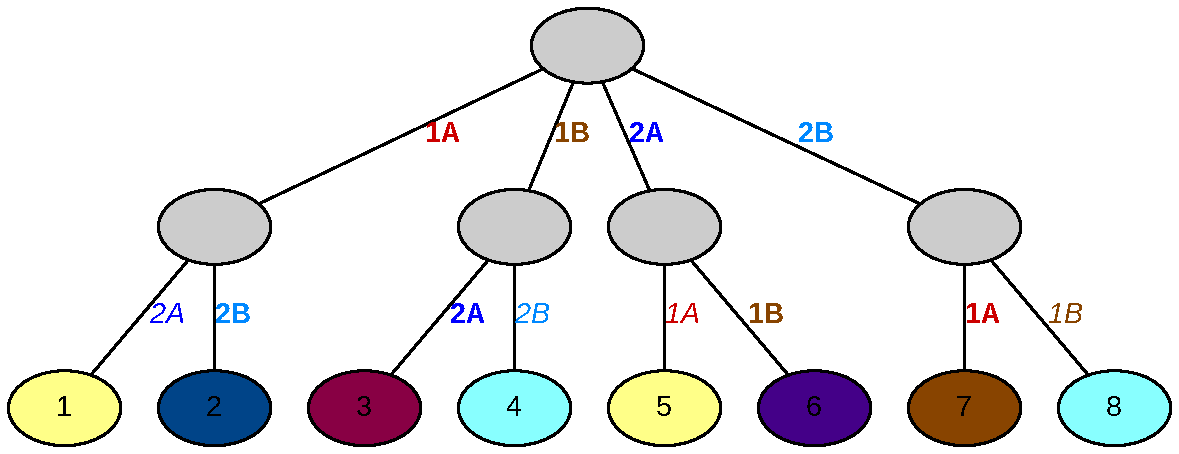
\includegraphics[width=0.8\textwidth]{htm-graph.pdf}
	\end{center}
	\caption{State space corresponding to the program in Figure~\ref{fig:txn-example}.
	Conflicting transitions are marked in bold;
	transitions which are independent from their predecessors are italicized.
	End states colored the same (the cyan and yellow ones) are equivalent.
	}
	\label{fig:txn-graph}
\end{figure}

\section{STM}

STM transactions abort only when multiple threads conflict.
Because Landslide already computes memory conflicts among each pair of transitions, it will be natural to extend DPOR to consult the conflict set when deciding whether to exercise a failure injection.
I will extend Landslide in this manner, and even support programs with both types of transactions, as long as the different {\tt xbegin} invocations are suitably annotated.

\section{Hybrid HTM/STM}

A recent paper \cite{hybrid-htm-stm} introduced several ways of combining HTM and STM in the same program, nesting transactions of different types.
It presented several semantics for such transactions transactions, the most interesting of which being ``open nesting'', in which a nested transaction's state becomes visible to other threads even during a containing transaction.
That state can then be rolled back if the latter aborts.
I plan to develop a theoretical model for how such transactions would affect Landslide's concurrency model,
although I expect to relegate any implementation thereof to future work.

\section{Evaluation Plan}

% TODO
